\documentclass[11pt]{article}
\usepackage[margin=18mm,headheight=22pt]{geometry}
\usepackage{amsmath}
\usepackage{fontspec}
\usepackage{unicode-math}
\setmainfont{NewCM10}[Extension=.otf,UprightFont=*-Book,BoldFont=*-Bold,ItalicFont=*-BookItalic,BoldItalicFont=*-BoldItalic]
\setsansfont{NewCMSans10}[Extension=.otf,UprightFont=*-Book,BoldFont=*-Bold,ItalicFont=*-BookOblique,BoldItalicFont=*-BoldOblique]
\setmathfont{NewCMMath-Book.otf}
\usepackage{xcolor}
\definecolor{FAUblue}{HTML}{04316A}
\definecolor{Paperblue}{HTML}{EEF2F7}
\definecolor{EEIgold}{HTML}{CC9C42}
\usepackage{etoolbox,enumitem,booktabs,tabularx,array,needspace,microtype}
\usepackage[most]{tcolorbox}
\usepackage{titlesec,fancyhdr}
\usepackage[hidelinks]{hyperref}
\usepackage{draftwatermark}
\SetWatermarkText{Made by Thanate Amornjiraporn (Focus)}
\SetWatermarkColor{black!7}\SetWatermarkFontSize{30pt}\SetWatermarkAngle{45}
\setlength{\parindent}{0pt}
\setlength{\parskip}{5pt}
\setlist{itemsep=2pt,topsep=3pt,leftmargin=1.6em,beginpenalty=10000,endpenalty=10000}
\raggedbottom
\clubpenalty=10000 \widowpenalty=10000 \displaywidowpenalty=10000 \interlinepenalty=10000
\setcounter{secnumdepth}{0}
\setcounter{tocdepth}{1}
\pagestyle{fancy}\fancyhf{}
\fancyhead[L]{\small\sffamily\color{FAUblue} From Fundamentals to AI Apocalypse · MEI · Chapter 3}
\fancyhead[R]{\small\sffamily Mappings and Elementary Functions}
\fancyfoot[C]{\small\thepage}
\titleformat{\section}{\Large\bfseries\sffamily\color{FAUblue}}{}{0pt}{}
\titleformat{\subsection}{\large\bfseries\sffamily\color{FAUblue}}{}{0pt}{}
\titlespacing*{\section}{0pt}{16pt}{6pt}
\preto\section{\Needspace{8\baselineskip}}
\preto\subsection{\Needspace{6\baselineskip}}
\newtcolorbox{equationcard}[1]{colback=Paperblue,colframe=Paperblue,boxrule=0pt,arc=0pt,left=10pt,right=10pt,top=6pt,bottom=6pt,title={#1},fonttitle=\small\bfseries\sffamily,coltitle=FAUblue,before skip=8pt,after skip=8pt}
\newtcolorbox{workedbox}[1]{colback=white,colframe=EEIgold,boxrule=0pt,leftrule=3pt,arc=0pt,left=10pt,top=4pt,bottom=4pt,title={#1},fonttitle=\small\bfseries\sffamily,coltitle=FAUblue,attach title to upper={\par},before skip=8pt,after skip=8pt}
\newtcolorbox{recallbox}[1]{colback=white,colframe=FAUblue,boxrule=0pt,leftrule=3pt,arc=0pt,left=10pt,top=4pt,bottom=4pt,title={#1},fonttitle=\small\bfseries\sffamily,coltitle=FAUblue,attach title to upper={\par},before skip=8pt,after skip=8pt}
\usepackage{environ}
\newsavebox\measurebox
% Typeset the section once invisibly to measure it; start a new page if it will not fit in what is left.
\makeatletter
\newif\ifkeep@measuring
\NewEnviron{keepsection}{%
  \ifkeep@measuring \BODY \else
    \edef\keep@sec{\the\value{section}}\edef\keep@sub{\the\value{subsection}}%
    \setbox\measurebox\vbox{\hsize\linewidth\keep@measuringtrue\def\Needspace##1{}\BODY}%
    \setcounter{section}{\keep@sec}\setcounter{subsection}{\keep@sub}%
    \dimen2=\ht\measurebox \advance\dimen2\dp\measurebox
    \dimen@=\textheight
    \ifdim\pagegoal<\maxdimen
      \dimen@=\pagegoal \advance\dimen@-\pagetotal
      \ifdim\dimen2>\dimen@ \clearpage \dimen@=\textheight \fi
    \fi
    % if it fits, nothing inside may force an early break
    \ifdim\dimen2>\dimen@ \BODY \else \begingroup\def\Needspace##1{}\BODY\endgroup \fi
  \fi}
\makeatother
\newtcolorbox{notebox}{colback=Paperblue,colframe=Paperblue,boxrule=0pt,arc=0pt,left=8pt,right=8pt,top=4pt,bottom=4pt,before skip=6pt,after skip=6pt}
\newtcolorbox{plainbox}{colback=white,colframe=FAUblue,boxrule=0pt,leftrule=3pt,arc=0pt,left=10pt,right=8pt,top=4pt,bottom=4pt,before skip=6pt,after skip=8pt}
\usetikzlibrary{arrows.meta}
\title{\sffamily\bfseries\color{FAUblue}Mappings and Elementary Functions}
\author{Mathematics for Engineers I \ensuremath{\cdot} Module 62765 \ensuremath{\cdot} Chapter 3\\[2pt]\small From Fundamentals to AI Apocalypse · personal study guide}
\date{}
\begin{document}
\maketitle
\begingroup\footnotesize\setlength{\parskip}{0pt}\tableofcontents\endgroup
\clearpage

\Needspace{9\baselineskip}
{\large This chapter builds the language of functions: how to describe mappings, test whether they have inverses, and combine them. It then applies that language to polynomials, trigonometric and exponential functions, and polar coordinates.}


\begin{keepsection}
\Needspace{16\baselineskip}
\section{Start from memory}

\Needspace{13\baselineskip}
Try these before reading. Write an answer even if you are uncertain; the gap tells you what to look for.

\Needspace{10\baselineskip}
\begin{enumerate}
\item What must be true for a rule from X to Y to be a mapping?
\item How do injective and surjective describe a mapping?
\item When does an inverse function exist?
\item In what order do you apply the functions in g\ensuremath{\circ}f?
\item What does the discriminant tell you about a quadratic’s real roots?
\item How do polar coordinates convert to Cartesian coordinates?
\end{enumerate}

\nopagebreak[4]{\small\itshape Answers: see “Start from memory” under Answers at the end.}
\end{keepsection}

\begin{keepsection}
\Needspace{22\baselineskip}
\section{How to use this guide}

\Needspace{19\baselineskip}
Attempt before reading each worked solution. Then hide the guide and retrieve the method on a later day.

\Needspace{16\baselineskip}
\begin{enumerate}
\item \textbf{Day 0:} Do the cold start. Read §§3.1–3.2 and draw a mapping diagram that distinguishes domain, codomain and image.
\item \textbf{Day 1:} Read §§3.3–3.4. Re-solve the inverse and composition examples from a blank page, then try mixed practice 1–8.
\item \textbf{Day 3:} Study the polynomial and trigonometric parts of §3.5. Rebuild the quadratic formula derivation, then solve practice 9–16 without notes.
\item \textbf{About day 7:} Study exponentials, logarithms and §3.6. Shuffle practice 17–24 and explain aloud which domain or quadrant condition matters.
\item \textbf{About day 14:} Rebuild all listed derivations and retry every marked question. Complete the self-check only with evidence from unaided work.
\item \textbf{Before the exam:} Do both exam problems under time limits, then review only the skills your evidence shows are weak.
\end{enumerate}
\end{keepsection}

\begin{keepsection}
\Needspace{19\baselineskip}
\section{How the chapter fits together}

\Needspace{16\baselineskip}
Mappings give a precise language for inputs and outputs. Injectivity supports inverses, compatible domains support composition, and elementary functions provide the examples used in coordinate changes.

\Needspace{9\baselineskip}
\subsection{Measured \ensuremath{\cdot} examples and coordinates}

\Needspace{6\baselineskip}
\begin{itemize}
\item 
\Needspace{4\baselineskip}
\textbf{Domain, codomain and image} \hfill{\small\color{FAUblue}§3.1}

\Needspace{4\baselineskip}
f:X\ensuremath{\to}Y; Im(f)\ensuremath{\subseteq}Y

Rests on: assigning exactly one output to each input.

\item 
\Needspace{4\baselineskip}
\textbf{Elementary functions} \hfill{\small\color{FAUblue}§3.5}

\Needspace{4\baselineskip}
P(x), sin x, e\textsuperscript{x}, ln x

Rests on: domain, rule and range being stated together.

\end{itemize}

\Needspace{9\baselineskip}
\subsection{Defined \ensuremath{\cdot} structure and operations}

\Needspace{6\baselineskip}
\begin{itemize}
\item 
\Needspace{4\baselineskip}
\textbf{Injective, surjective, bijective} \hfill{\small\color{FAUblue}§3.2}

\Needspace{4\baselineskip}
one-to-one; onto; both

Rests on: comparing the image with the codomain.

\item 
\Needspace{4\baselineskip}
\textbf{Composition} \hfill{\small\color{FAUblue}§3.4}

\Needspace{4\baselineskip}
(g\ensuremath{\circ}f)(x)=g(f(x))

Rests on: Im(f) fitting inside D(g).

\item 
\Needspace{4\baselineskip}
\textbf{Polar coordinates} \hfill{\small\color{FAUblue}§3.6}

\Needspace{4\baselineskip}
x=r cos φ, y=r sin φ

Rests on: sine and cosine on the unit circle.

\end{itemize}

\Needspace{8\baselineskip}
\subsection{Derived \ensuremath{\cdot} reversible and reusable results}

\Needspace{5\baselineskip}
\begin{itemize}
\item 
\Needspace{4\baselineskip}
\textbf{Inverse function} \hfill{\small\color{FAUblue}§3.3}

\Needspace{4\baselineskip}
f\textsuperscript{\ensuremath{-}1}\ensuremath{\circ}f=id\textsubscript{X}

Rests on: injectivity, so each reached output has one input.

\item 
\Needspace{4\baselineskip}
\textbf{Quadratic roots} \hfill{\small\color{FAUblue}§3.5}

\Needspace{4\baselineskip}
Δ=b\textsuperscript{2}\ensuremath{-}4ac

Rests on: completing the square and checking Δ’s sign.

\item 
\Needspace{4\baselineskip}
\textbf{Cartesian conversion} \hfill{\small\color{FAUblue}§3.6}

\Needspace{4\baselineskip}
r=\ensuremath{\surd}(x\textsuperscript{2}+y\textsuperscript{2})

Rests on: right-triangle length and a quadrant-aware angle.

\end{itemize}

\begin{keepsection}
\Needspace{15\baselineskip}
\subsection{Choose a tool}

\Needspace{10\baselineskip}
\begin{center}\small\begin{tabularx}{\linewidth}{>{\raggedright\arraybackslash}X>{\raggedright\arraybackslash}X}\toprule
\textbf{If the task asks…} & \textbf{Choose this tool} \\ \midrule
Does a rule define a function? & Check that each domain input has exactly one output. \\
Can you reverse the mapping? & Test injectivity, then solve y=f(x) for x. \\
What is f after g? & Write the composition order and check the intermediate domain. \\
How many real roots can a polynomial have? & Use degree for a bound; use Δ for a quadratic. \\
Where is an angle or point? & Use the unit circle or quadrant-aware polar conversion. \\
\bottomrule\end{tabularx}\end{center}
\end{keepsection}
\end{keepsection}

\begin{keepsection}
\Needspace{11\baselineskip}
\section{3.1 The Graph of a Mapping}

\Needspace{8\baselineskip}
A function is more than a formula: its domain and codomain are part of its definition. This lets you ask exactly which outputs occur and which inputs lead to a chosen set of outputs.

\Needspace{12\baselineskip}
\begin{plainbox}\textbf{In plain words:} think of a mapping as a machine with an input tray \textit{X} and an output tray \textit{Y}. Every input you drop in comes out as exactly one output. Two inputs may come out the same, and some outputs may never appear at all. The outputs that do appear form the \textbf{image}; the inputs whose output lands in a chosen set \textit{B} form the \textbf{preimage} of \textit{B}.\end{plainbox}

\begin{equationcard}{Mapping and image}
\[ \begin{gathered} {f}:{X}\to {Y} \\ \text{Im}({f})\, =\, \{{f}({x}):{x}\in {X}\}⊆{Y} \end{gathered} \]
{\small \emph{Read it as: “f maps X to Y”, and “the image of f is the set of all f(x) as x runs through X; it lies inside Y”.}\par X is the domain; Y is the codomain; Im(f) is the image or range. Every x\ensuremath{\in}X must be assigned exactly one value f(x)\ensuremath{\in}Y.}
\end{equationcard}

\begin{equationcard}{Image, preimage and graph}
\[ \begin{gathered} {f}({A})\, =\, \{{f}({x}):{x}\in {A}\} \\ {f}^{-1}({B})\, =\, \{{x}\in {X}:{f}({x})\in {B}\} \\ \text{Gr}({f})\, =\, \{({x},{y})\in {X}\times {Y}:{y}\, =\, {f}({x})\} \end{gathered} \]
{\small \emph{Read it as: “f of A is the set of outputs of the inputs in A”; “the preimage of B is the set of x in X whose output lies in B”; “the graph of f is the set of pairs (x, y) in X \ensuremath{\times} Y with y = f(x)”.}\par A\ensuremath{\subseteq}X and B\ensuremath{\subseteq}Y. Preimage notation f\textsuperscript{\ensuremath{-}1}(B) is defined even when f has no inverse function.}
\end{equationcard}

\Needspace{14\baselineskip}
\begin{center}
\begin{minipage}[t]{0.465\linewidth}\centering
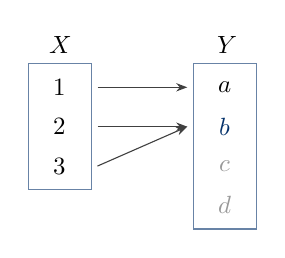
\begin{tikzpicture}[x=1cm,y=1cm,font=\small]
\draw[FAUblue!60] (0.00,0.3) rectangle (0.80,-1.30);
\node[above] at (0.40,0.3) {$X$};
\node[] at (0.40,0.00) {$1$};
\node[] at (0.40,-0.50) {$2$};
\node[] at (0.40,-1.00) {$3$};
\draw[FAUblue!60] (2.10,0.3) rectangle (2.90,-1.80);
\node[above] at (2.50,0.3) {$Y$};
\node[] at (2.50,0.00) {$a$};
\node[text=FAUblue,font=\small\bfseries] at (2.50,-0.50) {$b$};
\node[text=black!40] at (2.50,-1.00) {$c$};
\node[text=black!40] at (2.50,-1.50) {$d$};
\draw[-{Stealth[length=4pt]},black!75] (0.88,0.00) -- (2.02,0.00);
\draw[-{Stealth[length=4pt]},black!75] (0.88,-0.50) -- (2.02,-0.50);
\draw[-{Stealth[length=4pt]},black!75] (0.88,-1.00) -- (2.02,-0.50);
\end{tikzpicture}\par\smallskip{\small\raggedright \textbf{A mapping.} Exactly one arrow leaves every input. b is reached twice, and c and d never, so the image \{a, b\} is smaller than the codomain Y.\par}\end{minipage}\hfill
\begin{minipage}[t]{0.465\linewidth}\centering
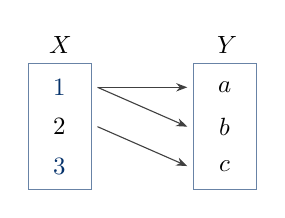
\begin{tikzpicture}[x=1cm,y=1cm,font=\small]
\draw[FAUblue!60] (0.00,0.3) rectangle (0.80,-1.30);
\node[above] at (0.40,0.3) {$X$};
\node[text=FAUblue,font=\small\bfseries] at (0.40,0.00) {$1$};
\node[] at (0.40,-0.50) {$2$};
\node[text=FAUblue,font=\small\bfseries] at (0.40,-1.00) {$3$};
\draw[FAUblue!60] (2.10,0.3) rectangle (2.90,-1.30);
\node[above] at (2.50,0.3) {$Y$};
\node[] at (2.50,0.00) {$a$};
\node[] at (2.50,-0.50) {$b$};
\node[] at (2.50,-1.00) {$c$};
\draw[-{Stealth[length=4pt]},black!75] (0.88,0.00) -- (2.02,0.00);
\draw[-{Stealth[length=4pt]},black!75] (0.88,0.00) -- (2.02,-0.50);
\draw[-{Stealth[length=4pt]},black!75] (0.88,-0.50) -- (2.02,-1.00);
\end{tikzpicture}\par\smallskip{\small\raggedright \textbf{Not a mapping.} 1 has two arrows and 3 has none; a mapping needs exactly one arrow from every input.\par}\end{minipage}
\end{center}

\Needspace{11\baselineskip}
A real-valued function has a graph in the coordinate plane. Each vertical line must meet the graph at most once: two y-values for one x would violate the mapping rule. A horizontal line may meet it more than once; that tells you the function is not injective, not that it fails to be a function.

\Needspace{13\baselineskip}
A rule need not be a single formula. The absolute value |x| splits into cases, and the Dirichlet function on [0,1] takes the value 1 at rational x and 0 at irrational x: it is a perfectly good mapping even though its graph cannot be drawn. A real-world assignment counts too, provided every input gets exactly one output, for example each product on a supermarket shelf gets exactly one price.

\begin{workedbox}{Worked example \ensuremath{\cdot} image and preimage}
Let f:\ensuremath{\mathbb{R}}\ensuremath{\to}\ensuremath{\mathbb{R}} be f(x)=x\textsuperscript{2}, and let A=\{\ensuremath{-}2,0,3\}, B=\{4\}.

\Needspace{6\baselineskip}
\begin{enumerate}
\item Apply the rule to each member of A: f(A)=\{4,0,9\}.
\item To find f\textsuperscript{\ensuremath{-}1}(B), solve x\textsuperscript{2}=4 over the stated domain \ensuremath{\mathbb{R}}. Both x=\ensuremath{-}2 and x=2 work, so f\textsuperscript{\ensuremath{-}1}(\{4\})=\{\ensuremath{-}2,2\}.
\item The image is [0,\ensuremath{\infty}), which is smaller than the codomain \ensuremath{\mathbb{R}}. Check: a square cannot be negative.
\end{enumerate}
\end{workedbox}

\Needspace{7\baselineskip}
\begin{notebox}\textbf{Trap:} f\textsuperscript{\ensuremath{-}1}(B) means “inputs that land in B”; it does not mean “apply the inverse function”. The inverse function exists only if f is injective.\end{notebox}

\Needspace{6\baselineskip}
\begin{notebox}\textbf{Near miss:} the rule “\textit{x} \ensuremath{\mapsto} \ensuremath{\pm}\ensuremath{\surd}\textit{x}” on [0, \ensuremath{\infty}) looks like a function, but it sends 4 to both 2 and \ensuremath{-}2. Two outputs for one input break the mapping rule; keeping only the positive root, \textit{x} \ensuremath{\mapsto} \ensuremath{\surd}\textit{x}, makes it a mapping.\end{notebox}

\Needspace{9\baselineskip}
\begin{recallbox}{Recall check \ensuremath{\cdot} answer before opening}
\Needspace{4\baselineskip}
\begin{enumerate}
\item What three sets are involved in f:X\ensuremath{\to}Y?
\item Can a preimage be defined when f is not injective?
\end{enumerate}

\nopagebreak[4]{\small\itshape Answers: see “3.1 The Graph of a Mapping” under Answers at the end.}
\end{recallbox}
\end{keepsection}

\begin{keepsection}
\Needspace{11\baselineskip}
\section{3.2 Types of Mappings}

\Needspace{8\baselineskip}
Injectivity and surjectivity answer different questions. Together they determine whether every output has exactly one input.

\Needspace{11\baselineskip}
\begin{plainbox}\textbf{In plain words:} picture the arrows from \textit{X} to \textit{Y}. \textbf{Injective} means no point of \textit{Y} receives two arrows: different inputs never share an output. \textbf{Surjective} means every point of \textit{Y} receives at least one arrow: nothing in the codomain is left out. \textbf{Bijective} means both, so inputs and outputs pair up one to one.\end{plainbox}

\begin{equationcard}{Injective}
\[ \begin{gathered} {x}_{1}\, ≠\, {x}_{2}\, \Rightarrow \, {f}({x}_{1})\, ≠\, {f}({x}_{2}) \end{gathered} \]
{\small \emph{Read it as: “if x\textsubscript{1} is not x\textsubscript{2}, then f(x\textsubscript{1}) is not f(x\textsubscript{2})”: different inputs always give different outputs.}\par Distinct inputs have distinct outputs; equivalently, f(x\textsubscript{1})=f(x\textsubscript{2}) implies x\textsubscript{1}=x\textsubscript{2}.}
\end{equationcard}

\begin{equationcard}{Surjective and bijective}
\[ \begin{gathered} {f}\, \text{is}\, \text{onto}\, {Y}\, \text{iff}\, \text{Im}({f})\, =\, {Y} \\ \text{bijective}\, \text{iff}\, \text{injective}\, \text{and}\, \text{surjective} \end{gathered} \]
{\small \emph{Read it as: “f is onto Y if and only if its image is all of Y”, and “bijective means injective and surjective at once”.}\par Surjectivity depends on the chosen codomain. A function is always surjective when its codomain is restricted to its image. Injectivity, in contrast, depends only on the graph \{(x,f(x)):x\ensuremath{\in}X\}: changing the codomain never changes it.}
\end{equationcard}

\Needspace{14\baselineskip}
\begin{center}
\begin{minipage}[t]{0.223\linewidth}\centering
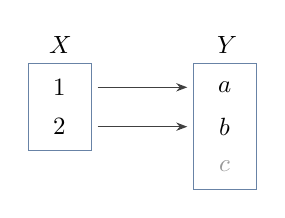
\begin{tikzpicture}[x=1cm,y=1cm,font=\small]
\draw[FAUblue!60] (0.00,0.3) rectangle (0.80,-0.80);
\node[above] at (0.40,0.3) {$X$};
\node[] at (0.40,0.00) {$1$};
\node[] at (0.40,-0.50) {$2$};
\draw[FAUblue!60] (2.10,0.3) rectangle (2.90,-1.30);
\node[above] at (2.50,0.3) {$Y$};
\node[] at (2.50,0.00) {$a$};
\node[] at (2.50,-0.50) {$b$};
\node[text=black!40] at (2.50,-1.00) {$c$};
\draw[-{Stealth[length=4pt]},black!75] (0.88,0.00) -- (2.02,0.00);
\draw[-{Stealth[length=4pt]},black!75] (0.88,-0.50) -- (2.02,-0.50);
\end{tikzpicture}\par\smallskip{\small\raggedright \textbf{Injective, not surjective.} No output is shared, but c is never reached.\par}\end{minipage}\hfill
\begin{minipage}[t]{0.223\linewidth}\centering
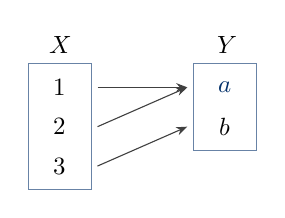
\begin{tikzpicture}[x=1cm,y=1cm,font=\small]
\draw[FAUblue!60] (0.00,0.3) rectangle (0.80,-1.30);
\node[above] at (0.40,0.3) {$X$};
\node[] at (0.40,0.00) {$1$};
\node[] at (0.40,-0.50) {$2$};
\node[] at (0.40,-1.00) {$3$};
\draw[FAUblue!60] (2.10,0.3) rectangle (2.90,-0.80);
\node[above] at (2.50,0.3) {$Y$};
\node[text=FAUblue,font=\small\bfseries] at (2.50,0.00) {$a$};
\node[] at (2.50,-0.50) {$b$};
\draw[-{Stealth[length=4pt]},black!75] (0.88,0.00) -- (2.02,0.00);
\draw[-{Stealth[length=4pt]},black!75] (0.88,-0.50) -- (2.02,0.00);
\draw[-{Stealth[length=4pt]},black!75] (0.88,-1.00) -- (2.02,-0.50);
\end{tikzpicture}\par\smallskip{\small\raggedright \textbf{Surjective, not injective.} Every output is reached, but a twice.\par}\end{minipage}\hfill
\begin{minipage}[t]{0.223\linewidth}\centering
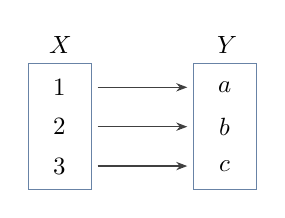
\begin{tikzpicture}[x=1cm,y=1cm,font=\small]
\draw[FAUblue!60] (0.00,0.3) rectangle (0.80,-1.30);
\node[above] at (0.40,0.3) {$X$};
\node[] at (0.40,0.00) {$1$};
\node[] at (0.40,-0.50) {$2$};
\node[] at (0.40,-1.00) {$3$};
\draw[FAUblue!60] (2.10,0.3) rectangle (2.90,-1.30);
\node[above] at (2.50,0.3) {$Y$};
\node[] at (2.50,0.00) {$a$};
\node[] at (2.50,-0.50) {$b$};
\node[] at (2.50,-1.00) {$c$};
\draw[-{Stealth[length=4pt]},black!75] (0.88,0.00) -- (2.02,0.00);
\draw[-{Stealth[length=4pt]},black!75] (0.88,-0.50) -- (2.02,-0.50);
\draw[-{Stealth[length=4pt]},black!75] (0.88,-1.00) -- (2.02,-1.00);
\end{tikzpicture}\par\smallskip{\small\raggedright \textbf{Bijective.} Every output is reached exactly once.\par}\end{minipage}\hfill
\begin{minipage}[t]{0.223\linewidth}\centering
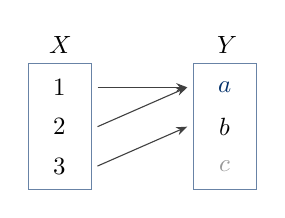
\begin{tikzpicture}[x=1cm,y=1cm,font=\small]
\draw[FAUblue!60] (0.00,0.3) rectangle (0.80,-1.30);
\node[above] at (0.40,0.3) {$X$};
\node[] at (0.40,0.00) {$1$};
\node[] at (0.40,-0.50) {$2$};
\node[] at (0.40,-1.00) {$3$};
\draw[FAUblue!60] (2.10,0.3) rectangle (2.90,-1.30);
\node[above] at (2.50,0.3) {$Y$};
\node[text=FAUblue,font=\small\bfseries] at (2.50,0.00) {$a$};
\node[] at (2.50,-0.50) {$b$};
\node[text=black!40] at (2.50,-1.00) {$c$};
\draw[-{Stealth[length=4pt]},black!75] (0.88,0.00) -- (2.02,0.00);
\draw[-{Stealth[length=4pt]},black!75] (0.88,-0.50) -- (2.02,0.00);
\draw[-{Stealth[length=4pt]},black!75] (0.88,-1.00) -- (2.02,-0.50);
\end{tikzpicture}\par\smallskip{\small\raggedright \textbf{Neither.} a is reached twice and c never.\par}\end{minipage}
\end{center}

\Needspace{12\baselineskip}
For f:\ensuremath{\mathbb{R}}\ensuremath{\to}\ensuremath{\mathbb{R}}, f(x)=x\textsuperscript{3} is strictly increasing and reaches every real value, so it is bijective. In contrast, x\textsuperscript{2} maps 1 and \ensuremath{-}1 to the same output and never reaches negative values: it is neither injective nor surjective onto \ensuremath{\mathbb{R}}. Restricting it to f:[0,\ensuremath{\infty})\ensuremath{\to}[0,\ensuremath{\infty}) makes it bijective.

\begin{workedbox}{Worked example \ensuremath{\cdot} the codomain changes surjectivity}
Consider f(x)=x\textsuperscript{2} with domain [0,\ensuremath{\infty}).

\Needspace{7\baselineskip}
\begin{enumerate}
\item If the codomain is \ensuremath{\mathbb{R}}, the mapping is injective but not surjective, because no negative real is a square.
\item If the codomain is [0,\ensuremath{\infty}), every codomain value y has the preimage \ensuremath{\surd}y. Thus it is surjective too.
\item So f:[0,\ensuremath{\infty})\ensuremath{\to}[0,\ensuremath{\infty}) is bijective. Check: each y\ensuremath{\geq}0 has exactly one non-negative square root.
\end{enumerate}
\end{workedbox}

\Needspace{6\baselineskip}
\begin{notebox}\textbf{Memory hook:} injective asks “does any output have two inputs?”; surjective asks “does any codomain value have no input?”. State the codomain before answering.\end{notebox}

\Needspace{5\baselineskip}
\begin{notebox}\textbf{Near miss:} \textit{f}(\textit{x}) = \textit{x}\textsuperscript{2} on [\ensuremath{-}1, \ensuremath{\infty}) is almost injective. On [0, \ensuremath{\infty}) it is, but \ensuremath{-}1 and 1 both give 1, and one shared output is enough to fail.\end{notebox}

\Needspace{10\baselineskip}
\begin{recallbox}{Recall check \ensuremath{\cdot} answer before opening}
\Needspace{4\baselineskip}
\begin{enumerate}
\item What is the difference between injective and surjective?
\item Why is x\ensuremath{\mapsto}x\textsuperscript{2} not onto \ensuremath{\mathbb{R}}?
\end{enumerate}

\nopagebreak[4]{\small\itshape Answers: see “3.2 Types of Mappings” under Answers at the end.}
\end{recallbox}
\end{keepsection}

\begin{keepsection}
\Needspace{11\baselineskip}
\section{3.3 Inverse Function}

\Needspace{8\baselineskip}
An inverse undoes a mapping. It can do that consistently only when an output identifies one input.

\Needspace{12\baselineskip}
\begin{plainbox}\textbf{In plain words:} the inverse runs the machine backwards: hand it an output and it returns the one input that produced it. That is only possible when no output came from two inputs (the mapping is injective), and it only accepts outputs that actually occur, which is why its domain is the image.\end{plainbox}

\begin{equationcard}{Inverse function}
\[ \begin{gathered} {f}:{X}\to {Y}\, \text{injective}\, \Rightarrow \, {f}^{-1}:\text{Im}({f})\to {X} \end{gathered} \]
{\small \emph{Read it as: “if f from X to Y is injective, then f inverse goes from the image of f back to X”.}\par For y\ensuremath{\in}Im(f), f\textsuperscript{\ensuremath{-}1}(y) is the unique x\ensuremath{\in}X satisfying f(x)=y. The inverse domain is Im(f), not necessarily all of Y.}
\end{equationcard}

\begin{equationcard}{Inverse identities}
\[ \begin{gathered} {f}^{-1}\circ {f}\, =\, \text{id}_{{X}} \\ {f}\circ {f}^{-1}\, =\, \text{id}_{\text{Im}({f})} \end{gathered} \]
{\small \emph{Read it as: “f inverse after f is the identity on X”: doing f and then undoing it gives back every x. “f after f inverse is the identity on the image of f.”}\par The domain and image switch. For real-valued functions, the two graphs reflect across y=x.}
\end{equationcard}

\Needspace{14\baselineskip}
\begin{center}
\begin{minipage}[t]{0.465\linewidth}\centering
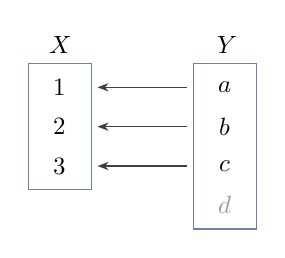
\begin{tikzpicture}[x=1cm,y=1cm,font=\small]
\draw[FAUblue!60] (0.00,0.3) rectangle (0.80,-1.30);
\node[above] at (0.40,0.3) {$X$};
\node[] at (0.40,0.00) {$1$};
\node[] at (0.40,-0.50) {$2$};
\node[] at (0.40,-1.00) {$3$};
\draw[FAUblue!60] (2.10,0.3) rectangle (2.90,-1.80);
\node[above] at (2.50,0.3) {$Y$};
\node[] at (2.50,0.00) {$a$};
\node[] at (2.50,-0.50) {$b$};
\node[] at (2.50,-1.00) {$c$};
\node[text=black!40] at (2.50,-1.50) {$d$};
\draw[-{Stealth[length=4pt]},black!75] (2.02,0.00) -- (0.88,0.00);
\draw[-{Stealth[length=4pt]},black!75] (2.02,-0.50) -- (0.88,-0.50);
\draw[-{Stealth[length=4pt]},black!75] (2.02,-1.00) -- (0.88,-1.00);
\end{tikzpicture}\par\smallskip{\small\raggedright \textbf{f\textsuperscript{\ensuremath{-}1} reverses every arrow.} It is defined on the image \{a, b, c\}; d is outside the image, so nothing leads back from it.\par}\end{minipage}\hfill
\begin{minipage}[t]{0.465\linewidth}\centering
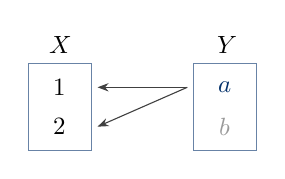
\begin{tikzpicture}[x=1cm,y=1cm,font=\small]
\draw[FAUblue!60] (0.00,0.3) rectangle (0.80,-0.80);
\node[above] at (0.40,0.3) {$X$};
\node[] at (0.40,0.00) {$1$};
\node[] at (0.40,-0.50) {$2$};
\draw[FAUblue!60] (2.10,0.3) rectangle (2.90,-0.80);
\node[above] at (2.50,0.3) {$Y$};
\node[text=FAUblue,font=\small\bfseries] at (2.50,0.00) {$a$};
\node[text=black!40] at (2.50,-0.50) {$b$};
\draw[-{Stealth[length=4pt]},black!75] (2.02,0.00) -- (0.88,0.00);
\draw[-{Stealth[length=4pt]},black!75] (2.02,0.00) -- (0.88,-0.50);
\end{tikzpicture}\par\smallskip{\small\raggedright \textbf{No inverse.} Reversing f would send a back to both 1 and 2, which is not a mapping.\par}\end{minipage}
\end{center}

\Needspace{10\baselineskip}
To find an inverse, write y=f(x), solve for x, then rename the output variable. Keep the domain restrictions: the inverse is defined only for values in the original image. Check both compositions when the domains allow it.

\begin{workedbox}{Worked example \ensuremath{\cdot} solve for the inverse}
Let f:\ensuremath{\mathbb{R}}\ensuremath{\to}\ensuremath{\mathbb{R}}, f(x)=2x+3.

\Needspace{5\baselineskip}
\begin{enumerate}
\item Set y=2x+3 and solve: x=(y\ensuremath{-}3)/2.
\item Therefore f\textsuperscript{\ensuremath{-}1}(y)=(y\ensuremath{-}3)/2, with domain \ensuremath{\mathbb{R}}.
\item Check: f\textsuperscript{\ensuremath{-}1}(f(x))=((2x+3)\ensuremath{-}3)/2=x. Also f(f\textsuperscript{\ensuremath{-}1}(y))=2((y\ensuremath{-}3)/2)+3=y.
\end{enumerate}
\end{workedbox}

\Needspace{6\baselineskip}
\begin{notebox}\textbf{Trap:} f\textsuperscript{\ensuremath{-}1}(x) is not 1/f(x). It means the inverse mapping. If f is not injective, solving y=f(x) may give multiple x-values and no inverse function.\end{notebox}

\Needspace{5\baselineskip}
\begin{notebox}\textbf{Near miss:} \textit{f}(\textit{x}) = \textit{x}\textsuperscript{2} on \ensuremath{\mathbb{R}} cannot be inverted: 2 and \ensuremath{-}2 both give 4, so “the input that gave 4” is not unique. Restrict the domain to [0, \ensuremath{\infty}) and it becomes injective, with \textit{f}\textsuperscript{\ensuremath{-}1}(\textit{y}) = \ensuremath{\surd}\textit{y}.\end{notebox}

\Needspace{9\baselineskip}
\begin{recallbox}{Recall check \ensuremath{\cdot} answer before opening}
\Needspace{4\baselineskip}
\begin{enumerate}
\item What is the domain of f\textsuperscript{\ensuremath{-}1}?
\item How can you check a proposed inverse?
\end{enumerate}

\nopagebreak[4]{\small\itshape Answers: see “3.3 Inverse Function” under Answers at the end.}
\end{recallbox}
\end{keepsection}

\begin{keepsection}
\Needspace{10\baselineskip}
\section{3.4 Composition}

\Needspace{7\baselineskip}
Composition chains mappings. The output of the first mapping must be a valid input to the next.

\Needspace{11\baselineskip}
\begin{plainbox}\textbf{In plain words:} composition is running one machine after another: \textit{f} first, then \textit{g} on whatever \textit{f} produced. The notation \textit{g} \ensuremath{\circ} \textit{f} is read from right to left, exactly like \textit{g}(\textit{f}(\textit{x})). It only works if every output of \textit{f} is something \textit{g} accepts.\end{plainbox}

\begin{equationcard}{Composition}
\[ \begin{gathered} \text{If}\, {f}:{X}\to {Y},\, {g}:{D}({g})⊆{Y}\to {Z},\, \text{and}\, \text{Im}({f})⊆{D}({g}),\, \text{then}\, ({g}\circ {f})({x})\, =\, {g}({f}({x})) \end{gathered} \]
{\small \emph{Read it as: “g after f, applied to x, equals g of f of x”. The function written next to x acts first.}\par Read right to left: apply f first, then g. The containment condition guarantees the second step is defined for every first-step output.}
\end{equationcard}

\Needspace{14\baselineskip}
\begin{center}
\begin{minipage}[t]{0.950\linewidth}\centering
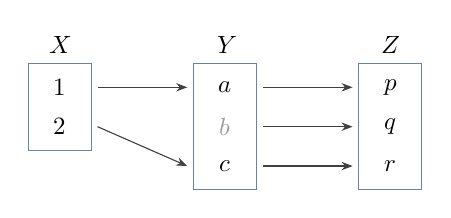
\begin{tikzpicture}[x=1cm,y=1cm,font=\small]
\draw[FAUblue!60] (0.00,0.3) rectangle (0.80,-0.80);
\node[above] at (0.40,0.3) {$X$};
\node[] at (0.40,0.00) {$1$};
\node[] at (0.40,-0.50) {$2$};
\draw[FAUblue!60] (2.10,0.3) rectangle (2.90,-1.30);
\node[above] at (2.50,0.3) {$Y$};
\node[] at (2.50,0.00) {$a$};
\node[text=black!40] at (2.50,-0.50) {$b$};
\node[] at (2.50,-1.00) {$c$};
\draw[FAUblue!60] (4.20,0.3) rectangle (5.00,-1.30);
\node[above] at (4.60,0.3) {$Z$};
\node[] at (4.60,0.00) {$p$};
\node[] at (4.60,-0.50) {$q$};
\node[] at (4.60,-1.00) {$r$};
\draw[-{Stealth[length=4pt]},black!75] (0.88,0.00) -- (2.02,0.00);
\draw[-{Stealth[length=4pt]},black!75] (0.88,-0.50) -- (2.02,-1.00);
\draw[-{Stealth[length=4pt]},black!75] (2.98,0.00) -- (4.12,0.00);
\draw[-{Stealth[length=4pt]},black!75] (2.98,-0.50) -- (4.12,-0.50);
\draw[-{Stealth[length=4pt]},black!75] (2.98,-1.00) -- (4.12,-1.00);
\end{tikzpicture}\par\smallskip{\small\raggedright \textbf{g \ensuremath{\circ} f follows two arrows.} 1 \ensuremath{\to} a \ensuremath{\to} p and 2 \ensuremath{\to} c \ensuremath{\to} r, so (g \ensuremath{\circ} f)(1) = p and (g \ensuremath{\circ} f)(2) = r. f never reaches b, so its arrow plays no part.\par}\end{minipage}
\end{center}

\begin{equationcard}{Composition laws}
\[ \begin{gathered} {h}\circ ({g}\circ {f})\, =\, ({h}\circ {g})\circ {f} \\ \text{in}\, \text{general}\, {g}\circ {f}\, ≠\, {f}\circ {g} \end{gathered} \]
{\small \emph{Read it as: “h after (g after f) equals (h after g) after f”, but “g after f is in general not f after g”.}\par Composition is associative when the domains fit, but order usually matters. For a bijection, f\textsuperscript{\ensuremath{-}1}\ensuremath{\circ}f=id\textsubscript{X}.}
\end{equationcard}

\begin{workedbox}{Worked example \ensuremath{\cdot} order and domain}
Let f:\ensuremath{\mathbb{R}}\ensuremath{\to}\ensuremath{\mathbb{R}} be f(x)=2x+1 and g:\ensuremath{\mathbb{R}}\ensuremath{\to}\ensuremath{\mathbb{R}} be g(x)=x\textsuperscript{2}.

\Needspace{6\baselineskip}
\begin{enumerate}
\item For g\ensuremath{\circ}f, apply f then square: (g\ensuremath{\circ}f)(x)=(2x+1)\textsuperscript{2}.
\item For f\ensuremath{\circ}g, square then apply f: (f\ensuremath{\circ}g)(x)=2x\textsuperscript{2}+1.
\item At x=1 these give 9 and 3, so the two compositions differ. This numerical check catches a reversed order.
\end{enumerate}
\end{workedbox}

\Needspace{6\baselineskip}
\begin{notebox}\textbf{Trap:} do not apply the left-hand function first. Write the nested expression g(f(x)) before simplifying, and check that f’s image lies in g’s domain.\end{notebox}

\Needspace{5\baselineskip}
\begin{notebox}\textbf{Near miss:} with \textit{f}(\textit{x}) = \textit{x} \ensuremath{-} 2 and \textit{g}(\textit{x}) = \ensuremath{\surd}\textit{x}, the composite \textit{g}(\textit{f}(\textit{x})) = \ensuremath{\surd}(\textit{x} \ensuremath{-} 2) is not defined on all of \ensuremath{\mathbb{R}}: \textit{f}(0) = \ensuremath{-}2 lies outside the domain [0, \ensuremath{\infty}) of \textit{g}. Restrict \textit{f} to [2, \ensuremath{\infty}) first.\end{notebox}

\Needspace{9\baselineskip}
\begin{recallbox}{Recall check \ensuremath{\cdot} answer before opening}
\Needspace{4\baselineskip}
\begin{enumerate}
\item In g\ensuremath{\circ}f, which mapping acts first?
\item What must be true for g\ensuremath{\circ}f to be defined on all of X?
\end{enumerate}

\nopagebreak[4]{\small\itshape Answers: see “3.4 Composition” under Answers at the end.}
\end{recallbox}
\end{keepsection}

\begin{keepsection}
\Needspace{12\baselineskip}
\section{3.5 Elementary Functions}

\Needspace{9\baselineskip}
This section collects important real-valued mappings. Their domain and range determine where inverse functions and formulas make sense.

\begin{plainbox}\textbf{In plain words:} this section is a toolbox of the standard functions you will use all year: polynomials, the trigonometric functions, and the exponential and logarithm. For each one, learn three facts: where it is defined, which values it takes, and where it is injective. The last fact decides where it has an inverse: the logarithm undoes the exponential, and arcsin undoes sin on [\ensuremath{-}π/2, π/2].\end{plainbox}

\begin{keepsection}
\Needspace{10\baselineskip}
\subsection{Real polynomials}

\begin{equationcard}{Polynomial and roots}
\[ \begin{gathered} {P}({x})\, =\, {a}_{{n}}{x}^{{n}}\, +\, …\, +\, {a}_{1}{x}\, +\, {a}_{0}, {a}_{{n}}\, ≠\, 0 \\ {P}({x}_{0})\, =\, 0\, \text{means}\, {x}_{0}\, \text{is}\, \mathrm{a}\, \text{root} \end{gathered} \]
{\small \emph{Read it as: “P of x is a sum of powers of x, from a\textsubscript{n} x to the n down to the constant a\textsubscript{0}, with a\textsubscript{n} not zero”.}\par The degree is n and the domain is \ensuremath{\mathbb{R}}. A degree-n polynomial has at most n real roots.}
\end{equationcard}

\begin{equationcard}{Quadratic formula and discriminant}
\[ \begin{gathered} Δ\, =\, {b}^{2}-4\text{ac} \\ {x}\, =\, (-{b}\pm \sqrtΔ)/(2{a}), \text{ax}^{2}+\text{bx}+{c}\, =\, 0,\, {a}\, ≠\, 0 \end{gathered} \]
{\small \emph{Read it as: “delta is b squared minus four a c”: its sign tells you how many real roots there are before you solve anything.}\par Δ\ensuremath{>}0 gives two distinct real roots; Δ=0 gives one repeated root; Δ\ensuremath{<}0 gives no real roots. When Δ\ensuremath{\geq}0, the roots factor the polynomial as a(x\ensuremath{-}x\textsubscript{1})(x\ensuremath{-}x\textsubscript{2}).}
\end{equationcard}

\Needspace{9\baselineskip}
Completing the square reveals why Δ controls the roots. Multiply the equation by 4a, add b\textsuperscript{2}, and rewrite the left side as (2ax+b)\textsuperscript{2}. Taking square roots creates a real solution only if Δ\ensuremath{\geq}0.

\begin{workedbox}{Worked example \ensuremath{\cdot} solve a quadratic}
Solve x\textsuperscript{2}\ensuremath{-}5x+6=0.

\Needspace{5\baselineskip}
\begin{enumerate}
\item Here a=1, b=\ensuremath{-}5, c=6, so Δ=(\ensuremath{-}5)\textsuperscript{2}\ensuremath{-}4\ensuremath{\cdot}1\ensuremath{\cdot}6=1.
\item The roots are (5\ensuremath{\pm}1)/2, hence x=2 or x=3.
\item Check by factoring: x\textsuperscript{2}\ensuremath{-}5x+6=(x\ensuremath{-}2)(x\ensuremath{-}3). Substitution gives zero at both roots.
\end{enumerate}
\end{workedbox}

\Needspace{8\baselineskip}
General root formulas exist for degrees 3 and 4. For degree 5 and above there is no general formula built from the coefficients using only +, \ensuremath{-}, \ensuremath{\times}, ÷ and roots (the Abel–Ruffini theorem); the notes say “no general formulas”, which is meant in this sense. This does not prevent a particular higher-degree polynomial from factoring or having roots found by another method.

\Needspace{6\baselineskip}
\begin{notebox}\textbf{Sign check:} for Δ\ensuremath{<}0 there are no real roots, but the polynomial still has a real graph. “No real roots” does not mean “no roots in every number system.”\end{notebox}

\begin{notebox}\textbf{Near miss:} \textit{x}\textsuperscript{2} + 1 = 0 looks as if it should have the roots \ensuremath{\pm}1, but Δ = 0 \ensuremath{-} 4 = \ensuremath{-}4 \ensuremath{<} 0, so it has no real roots. It is \textit{x}\textsuperscript{2} \ensuremath{-} 1 = 0, with Δ = 4, that has the roots \ensuremath{\pm}1.\end{notebox}
\end{keepsection}

\begin{keepsection}
\Needspace{9\baselineskip}
\subsection{Trigonometric functions}

\begin{equationcard}{Unit circle and radians}
\[ \begin{gathered} {P}\, =\, (\text{cos}\, {x},\text{sin}\, {x}) \\ \text{tan}\, {x}\, =\, \text{sin}\, {x}/\text{cos}\, {x} \end{gathered} \]
{\small Angles are in radians. One full turn is 2π radians = 360°. On a right triangle, sin x is opposite/hypotenuse and cos x is adjacent/hypotenuse for acute x.}
\end{equationcard}

\Needspace{14\baselineskip}
\begin{center}
\begin{minipage}[t]{0.950\linewidth}\centering
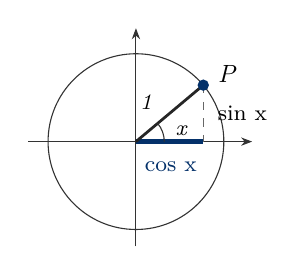
\begin{tikzpicture}
\draw[-{Stealth[length=4pt]},black!80] (0.144,-1.512) -- (2.988,-1.512);
\draw[-{Stealth[length=4pt]},black!80] (1.512,-2.844) -- (1.512,-0.072);
\draw[black!80] (1.512,-1.512) circle (1.116);
\draw[black!60,dashed] (2.367,-0.795) -- (2.367,-1.512);
\draw[FAUblue,line width=2pt] (1.512,-1.512) -- (2.367,-1.512);
\draw[black!85,line width=1pt] (1.512,-1.512) -- (2.367,-0.795);
\draw[black!80] (1.872,-1.512) arc (0:40.0:0.360);
\fill[FAUblue] (2.367,-0.795) circle (0.072);
\node[,inner sep=1pt,font=\footnotesize] at (2.094,-1.376) {\textit{x}};
\node[anchor=west,text=FAUblue,inner sep=1pt,font=\footnotesize] at (1.584,-1.836) {cos x};
\node[anchor=west,inner sep=1pt,font=\footnotesize] at (2.511,-1.153) {sin x};
\node[anchor=east,inner sep=1pt,font=\footnotesize] at (1.759,-1.009) {\textit{1}};
\node[anchor=west,inner sep=1pt,font=\small] at (2.511,-0.651) {\textit{P}};
\end{tikzpicture}\par\smallskip{\small\raggedright \textbf{The unit circle.} The point at angle \textit{x} on a circle of radius 1 is P = (cos \textit{x}, sin \textit{x}): cos \textit{x} is how far right, sin \textit{x} how far up.\par}\end{minipage}
\end{center}

\Needspace{10\baselineskip}
\begin{center}\small\begin{tabularx}{\linewidth}{>{\raggedright\arraybackslash}X>{\raggedright\arraybackslash}X>{\raggedright\arraybackslash}X>{\raggedright\arraybackslash}X>{\raggedright\arraybackslash}X>{\raggedright\arraybackslash}X>{\raggedright\arraybackslash}X>{\raggedright\arraybackslash}X}\toprule
\textbf{Degrees} & \textbf{0°} & \textbf{30°} & \textbf{45°} & \textbf{60°} & \textbf{90°} & \textbf{180°} & \textbf{360°} \\ \midrule
\textbf{Radians} & \textbf{0} & \textbf{π/6} & \textbf{π/4} & \textbf{π/3} & \textbf{π/2} & \textbf{π} & \textbf{2π} \\ \midrule
\bottomrule\end{tabularx}\end{center}

\begin{equationcard}{Core trigonometric identities}
\[ \begin{gathered} \text{sin}(-{x})\, =\, -\text{sin}\, {x} \\ \text{cos}(-{x})\, =\, \text{cos}\, {x} \\ \text{sin}^{2}{x}+\text{cos}^{2}{x}\, =\, 1 \\ \text{sin}({x}\pm {y})\, =\, \text{sin}\, {x}\, \text{cos}\, {y}\pm \text{cos}\, {x}\, \text{sin}\, {y} \\ \text{cos}({x}\pm {y})\, =\, \text{cos}\, {x}\, \text{cos}\, {y}\mp \text{sin}\, {x}\, \text{sin}\, {y} \end{gathered} \]
{\small sin and cos have period 2π. Their zeros are sin x=0 at x=kπ and cos x=0 at x=π/2+kπ, k\ensuremath{\in}\ensuremath{\mathbb{Z}}.}
\end{equationcard}

\begin{equationcard}{Shifts and periodicity}
\[ \begin{gathered} \text{sin}({x}+π/2)\, =\, \text{cos}\, {x} \\ \text{cos}({x}+π/2)\, =\, -\text{sin}\, {x} \\ \text{sin}({x}+π)\, =\, -\text{sin}\, {x} \\ \text{cos}({x}+π)\, =\, -\text{cos}\, {x} \\ \text{sin}({x}+2π)\, =\, \text{sin}\, {x} \\ \text{cos}({x}+2π)\, =\, \text{cos}\, {x} \end{gathered} \]
{\small Each follows from an addition formula with cos and sin of π/2, π or 2π. A quarter turn turns sine into cosine; a half turn flips both signs.}
\end{equationcard}

\begin{equationcard}{Double-angle and square identities}
\[ \begin{gathered} \text{sin}(2{x})\, =\, 2\, \text{sin}\, {x}\, \text{cos}\, {x} \\ \text{cos}(2{x})\, =\, 1-2\, \text{sin}^{2}{x}\, =\, 2\, \text{cos}^{2}{x}-1\, =\, \text{cos}^{2}{x}-\text{sin}^{2}{x} \\ \text{sin}^{2}{x}\, =\, (1-\text{cos}\, 2{x})/2 \\ \text{cos}^{2}{x}\, =\, (1+\text{cos}\, 2{x})/2 \end{gathered} \]
{\small These follow from the addition formulas and sin\textsuperscript{2}x+cos\textsuperscript{2}x=1.}
\end{equationcard}

\begin{equationcard}{Difference-to-product identities}
\[ \begin{gathered} \text{sin}\, {x}-\text{sin}\, {y}\, =\, 2\, \text{cos}(({x}+{y})/2)\, \text{sin}(({x}-{y})/2) \\ \text{cos}\, {x}-\text{cos}\, {y}\, =\, 2\, \text{sin}(({x}+{y})/2)\, \text{sin}(({y}-{x})/2) \end{gathered} \]
{\small The second factor uses (y\ensuremath{-}x)/2; reversing its sign would reverse the whole result.}
\end{equationcard}

\begin{workedbox}{Worked example \ensuremath{\cdot} use an addition formula}
Find sin(π/3+π/6).

\Needspace{5\baselineskip}
\begin{enumerate}
\item Use sin(x+y)=sin x cos y+cos x sin y.
\item Substitute the special-angle values: (\ensuremath{\surd}3/2)(\ensuremath{\surd}3/2)+(1/2)(1/2)=3/4+1/4=1.
\item The result matches sin(π/2)=1, a useful unit-circle check.
\end{enumerate}
\end{workedbox}

\Needspace{11\baselineskip}
For inverse functions, restrict sine to [\ensuremath{-}π/2,π/2], cosine to [0,π], and tangent to (\ensuremath{-}π/2,π/2). Then arcsin and arccos have domain [\ensuremath{-}1,1], while arctan has domain \ensuremath{\mathbb{R}}. tan x is undefined when cos x=0, that is x=π/2+kπ.

\begin{equationcard}{Tangent identities}
\[ \begin{gathered} \text{tan}(-{x})\, =\, -\text{tan}\, {x} \\ \text{tan}({x}\pm {y})\, =\, (\text{tan}\, {x}\pm \text{tan}\, {y})/(1\mp \text{tan}\, {x}\, \text{tan}\, {y}) \\ \text{tan}(2{x})\, =\, 2\, \text{tan}\, {x}/(1-\text{tan}^{2}{x}) \end{gathered} \]
{\small Use only where each tangent and denominator is defined. These follow by dividing the sine and cosine addition formulas.}
\end{equationcard}

\begin{notebox}\textbf{Trap:} inverse trigonometric functions return principal angles, not every angle with that sine or cosine. Check the interval and quadrant before giving a general solution.\end{notebox}
\end{keepsection}

\begin{keepsection}
\Needspace{9\baselineskip}
\subsection{Exponential and logarithmic functions}

\begin{equationcard}{Exponential and natural logarithm}
\[ \begin{gathered} {e}^{{x}+{y}}\, =\, {e}^{{x}}{e}^{{y}} \\ \text{ln}({e}^{{x}})\, =\, {x} \\ {e}^{\text{ln}\, {y}}\, =\, {y}\, \text{for}\, {y}\, >\, 0 \\ \text{ln}(\text{xy})\, =\, \text{ln}\, {x}+\text{ln}\, {y}\, \text{for}\, {x},{y}\, >\, 0 \\ \text{ln}\, 1\, =\, 0 \end{gathered} \]
{\small e\textsuperscript{x} is strictly increasing, positive, and has range (0,\ensuremath{\infty}). ln is its inverse, with domain (0,\ensuremath{\infty}).}
\end{equationcard}

\begin{equationcard}{Base a and real powers}
\[ \begin{gathered} {a}^{{x}}\, =\, {e}^{{x}\, \text{ln}\, {a}}\, ({a}\, >\, 0) \\ \text{log}_{{a}}{x}\, =\, \text{ln}\, {x}/\text{ln}\, {a}\, ({a}\, >\, 0,\, {a}\, ≠\, 1,\, {x}\, >\, 0) \\ {x}^{α}\, =\, {e}^{α\, \text{ln}\, {x}}\, \text{for}\, {x}\, >\, 0,\, α\in \mathbb{R} \end{gathered} \]
{\small For 0\ensuremath{<}a\ensuremath{<}1, a\textsuperscript{x} decreases; for a\ensuremath{>}1 it increases. The notes define arbitrary real powers x\textsuperscript{α} only for positive x.}
\end{equationcard}

\begin{workedbox}{Worked example \ensuremath{\cdot} solve an exponential equation}
Solve 5\textsuperscript{x}=125.

\Needspace{5\baselineskip}
\begin{enumerate}
\item Write 125=5\textsuperscript{3}, so 5\textsuperscript{x}=5\textsuperscript{3}.
\item Because the base 5 is positive and not 1, the exponential is injective. Therefore x=3.
\item Check: 5\textsuperscript{3}=125 and x is allowed in the domain \ensuremath{\mathbb{R}}.
\end{enumerate}
\end{workedbox}

\Needspace{5\baselineskip}
\begin{notebox}\textbf{Trap:} ln x is defined for x\ensuremath{>}0 only. Also, log\textsubscript{a} requires a\ensuremath{>}0 and a\ensuremath{\neq}1; a=1 would give a constant function with no inverse.\end{notebox}

\Needspace{10\baselineskip}
\begin{recallbox}{Recall check \ensuremath{\cdot} answer before opening}
\Needspace{5\baselineskip}
\begin{enumerate}
\item What does the sign of a quadratic’s discriminant tell you?
\item On which interval is sin restricted to define arcsin?
\item What are the domain and range of ln?
\end{enumerate}

\nopagebreak[4]{\small\itshape Answers: see “3.5 Elementary Functions” under Answers at the end.}
\end{recallbox}
\end{keepsection}
\end{keepsection}

\begin{keepsection}
\Needspace{11\baselineskip}
\section{3.6 Polar Coordinates}

\Needspace{8\baselineskip}
Cartesian coordinates locate a point by horizontal and vertical displacement. Polar coordinates use distance from the origin and angle from the positive x-axis.

\Needspace{12\baselineskip}
\begin{plainbox}\textbf{In plain words:} polar coordinates describe a point the way you give directions: how far to walk from the origin (\textit{r}) and in which direction (the angle φ, measured from the positive \textit{x}-axis). Cartesian coordinates say how far right and how far up. A right triangle with hypotenuse \textit{r} links the two.\end{plainbox}

\begin{equationcard}{Polar to Cartesian}
\[ \begin{gathered} {x}\, =\, {r}\, \text{cos}\, φ \\ {y}\, =\, {r}\, \text{sin}\, φ \end{gathered} \]
{\small \emph{Read it as: “x is r cos phi, y is r sin phi”: the horizontal and vertical sides of a right triangle with hypotenuse r and angle φ.}\par Here r\ensuremath{\geq}0 and φ is measured in radians from the positive x-axis. The point is (x,y)=(r cos φ,r sin φ).}
\end{equationcard}

\Needspace{14\baselineskip}
\begin{center}
\begin{minipage}[t]{0.950\linewidth}\centering
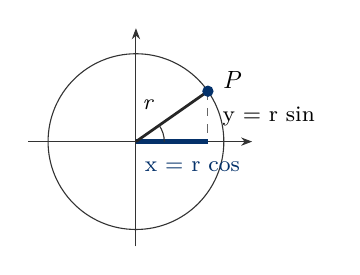
\begin{tikzpicture}
\draw[-{Stealth[length=4pt]},black!80] (0.144,-1.512) -- (2.988,-1.512);
\draw[-{Stealth[length=4pt]},black!80] (1.512,-2.844) -- (1.512,-0.072);
\draw[black!80] (1.512,-1.512) circle (1.116);
\draw[black!60,dashed] (2.426,-0.872) -- (2.426,-1.512);
\draw[FAUblue,line width=2pt] (1.512,-1.512) -- (2.426,-1.512);
\draw[black!85,line width=1pt] (1.512,-1.512) -- (2.426,-0.872);
\draw[black!80] (1.872,-1.512) arc (0:35.0:0.360);
\fill[FAUblue] (2.426,-0.872) circle (0.072);
\node[,inner sep=1pt,font=\footnotesize] at (2.101,-1.396) {\textit{φ}};
\node[anchor=west,text=FAUblue,inner sep=1pt,font=\footnotesize] at (1.584,-1.836) {x = r cos φ};
\node[anchor=west,inner sep=1pt,font=\footnotesize] at (2.570,-1.192) {y = r sin φ};
\node[anchor=east,inner sep=1pt,font=\footnotesize] at (1.789,-1.048) {\textit{r}};
\node[anchor=west,inner sep=1pt,font=\small] at (2.570,-0.728) {\textit{P}};
\end{tikzpicture}\par\smallskip{\small\raggedright \textbf{Polar to Cartesian.} For the point at distance \textit{r} and angle φ, the horizontal side of the triangle is \textit{r} cos φ and the vertical side \textit{r} sin φ.\par}\end{minipage}
\end{center}

\begin{equationcard}{Cartesian to polar}
\[ \begin{gathered} {r}\, =\, \sqrt({x}^{2}+{y}^{2}) \\ \text{tan}\, φ\, =\, {y}/{x}\, \text{when}\, {x}\, ≠\, 0 \end{gathered} \]
{\small \emph{Read it as: “r is the square root of x squared plus y squared” (Pythagoras), and “tan phi is y over x”, which fixes φ only up to the quadrant.}\par Use the signs of x and y to select the quadrant. For 0\ensuremath{\leq}φ\ensuremath{<}2π: use arctan(y/x) when x\ensuremath{>}0,y\ensuremath{\geq}0; add 2π when x\ensuremath{>}0,y\ensuremath{<}0; add π when x\ensuremath{<}0; take π/2 when x=0,y\ensuremath{>}0 and 3π/2 when x=0,y\ensuremath{<}0. The origin has r=0 and no unique angle.}
\end{equationcard}

\Needspace{12\baselineskip}
With r\ensuremath{\geq}0 and unrestricted angle, polar coordinates are not unique: adding 2π does not move the point, and the origin has every angle. Restricting to r\ensuremath{>}0 and 0\ensuremath{\leq}φ\ensuremath{<}2π gives one polar pair for every non-origin point. The origin must be handled separately if it is included.

\begin{workedbox}{Worked example \ensuremath{\cdot} convert a point and a region}
\Needspace{7\baselineskip}
\begin{enumerate}
\item Convert (x,y)=(\ensuremath{-}1,1). The radius is r=\ensuremath{\surd}(1+1)=\ensuremath{\surd}2. The point is in quadrant II, so φ=3π/4. Thus (\ensuremath{-}1,1)=(\ensuremath{\surd}2,3π/4).
\item Convert the region 0\ensuremath{\leq}r\ensuremath{\leq}2, 0\ensuremath{\leq}φ\ensuremath{\leq}π/4. Since r\textsuperscript{2}=x\textsuperscript{2}+y\textsuperscript{2}, it lies inside the circle x\textsuperscript{2}+y\textsuperscript{2}\ensuremath{\leq}4. The angle range is the first-quadrant wedge between y=0 and y=x, so 0\ensuremath{\leq}y\ensuremath{\leq}x.
\item Check a boundary point: r=2, φ=π/4 gives x=y=\ensuremath{\surd}2 and x\textsuperscript{2}+y\textsuperscript{2}=4.
\end{enumerate}
\end{workedbox}

\Needspace{7\baselineskip}
\begin{notebox}\textbf{Sign check:} arctan(y/x) alone returns an angle only in its principal range. Use the signs of both coordinates; when x=0, use the vertical-axis cases, and at the origin the angle is undefined.\end{notebox}

\Needspace{5\baselineskip}
\begin{notebox}\textbf{Near miss:} for (\textit{x}, \textit{y}) = (\ensuremath{-}1, \ensuremath{-}1), tan φ = 1 suggests φ = π/4, but that points into the first quadrant. Both coordinates are negative, so add π: φ = 5π/4.\end{notebox}

\Needspace{9\baselineskip}
\begin{recallbox}{Recall check \ensuremath{\cdot} answer before opening}
\Needspace{4\baselineskip}
\begin{enumerate}
\item What are x and y in terms of r and φ?
\item Why must you check the quadrant when finding φ?
\end{enumerate}

\nopagebreak[4]{\small\itshape Answers: see “3.6 Polar Coordinates” under Answers at the end.}
\end{recallbox}
\end{keepsection}

\begin{keepsection}
\Needspace{25\baselineskip}
\section{Formula map and checks}

\Needspace{22\baselineskip}
This chapter has no SI-valued quantities; domains, ranges and angle units (radians) take the place of physical units.

\Needspace{10\baselineskip}
\begin{center}\small\begin{tabularx}{\linewidth}{>{\raggedright\arraybackslash}X>{\raggedright\arraybackslash}X>{\raggedright\arraybackslash}X}\toprule
\textbf{Topic} & \textbf{Relation} & \textbf{Check} \\ \midrule
Image and preimage & Im(f)=\{f(x):x\ensuremath{\in}X\}; f\textsuperscript{\ensuremath{-}1}(B)=\{x:f(x)\ensuremath{\in}B\} & Keep image values in the codomain; preimage is not an inverse function. \\
Types & Injective: equal outputs imply equal inputs; onto: Im(f)=Y & State the codomain before deciding “onto”. \\
Inverse & f\textsuperscript{\ensuremath{-}1}:Im(f)\ensuremath{\to}X; f\textsuperscript{\ensuremath{-}1}\ensuremath{\circ}f=id\textsubscript{X} & Only for an injective mapping. \\
Composition & (g\ensuremath{\circ}f)(x)=g(f(x)) & f first; verify Im(f)\ensuremath{\subseteq}D(g). \\
Quadratic & Δ=b\textsuperscript{2}\ensuremath{-}4ac; x=(\ensuremath{-}b\ensuremath{\pm}\ensuremath{\surd}Δ)/(2a) & Use real-root cases by the sign of Δ; require a\ensuremath{\neq}0. \\
Trigonometry & sin\textsuperscript{2}x+cos\textsuperscript{2}x=1; sin(x\ensuremath{\pm}y)=sin x cos y\ensuremath{\pm}cos x sin y; cos(x\ensuremath{\pm}y)=cos x cos y\ensuremath{\mp}sin x sin y; sin(2x)=2 sin x cos x; sin x\ensuremath{-}sin y=2 cos((x+y)/2) sin((x\ensuremath{-}y)/2); tan(x\ensuremath{\pm}y)=(tan x\ensuremath{\pm}tan y)/(1\ensuremath{\mp}tan x tan y) & Angles are radians; exclude cosine or denominators equal to zero. \\
Exponential/logarithm & e\textsuperscript{x+y}=e\textsuperscript{x}e\textsuperscript{y}; ln(xy)=ln x+ln y; log\textsubscript{a}x=ln x/ln a & x,y\ensuremath{>}0 and a\ensuremath{>}0, a\ensuremath{\neq}1 for log\textsubscript{a}. \\
Polar conversion & x=r cos φ; y=r sin φ; r=\ensuremath{\surd}(x\textsuperscript{2}+y\textsuperscript{2}) & Angles are radians; check quadrant; origin has no unique angle. \\
\bottomrule\end{tabularx}\end{center}
\end{keepsection}

\begin{keepsection}
\Needspace{16\baselineskip}
\section{Derive it cold}

\Needspace{13\baselineskip}
Rebuild these on blank paper before opening the worked examples in the relevant sections.

\Needspace{11\baselineskip}
\begin{enumerate}
\item Show that the graph of a real-valued function meets each vertical line at most once. \hfill{\small\color{FAUblue}§3.1}
\item Derive the range of x\ensuremath{\mapsto}x\textsuperscript{2} on \ensuremath{\mathbb{R}} and show why it is not injective there. \hfill{\small\color{FAUblue}§3.2}
\item Starting from y=f(x), solve for x to obtain the inverse of a one-to-one affine function. \hfill{\small\color{FAUblue}§3.3}
\item Compute both g\ensuremath{\circ}f and f\ensuremath{\circ}g for f(x)=2x+1, g(x)=x\textsuperscript{2}, and compare. \hfill{\small\color{FAUblue}§3.4}
\item Complete the square in ax\textsuperscript{2}+bx+c=0 and derive the quadratic formula. \hfill{\small\color{FAUblue}§3.5}
\item Derive the double-angle formulas from the sine and cosine addition formulas. \hfill{\small\color{FAUblue}§3.5}
\item Derive x=r cos φ and y=r sin φ from a right triangle, then recover r by Pythagoras. \hfill{\small\color{FAUblue}§3.6}
\end{enumerate}
\end{keepsection}

\begin{keepsection}
\Needspace{19\baselineskip}
\section{Explain it}

\Needspace{16\baselineskip}
Answer aloud in complete sentences. Then compare with the model answer. (Retrieval and explanatory questioning [MIS, AMN, NEW].)

\Needspace{13\baselineskip}
\begin{enumerate}
\item \textbf{Why} is the codomain part of a function’s definition?
\item \textbf{When} can a mapping be surjective after changing only its codomain?
\item \textbf{Why} does an inverse function require injectivity?
\item \textbf{When} is g\ensuremath{\circ}f defined for every x in X?
\item \textbf{Why} does the discriminant determine the number of real quadratic roots?
\item \textbf{Why} must inverse trigonometric functions use restricted intervals?
\item \textbf{When} is log\textsubscript{a} x defined, and why can a not equal 1?
\item \textbf{Why} do polar coordinates need a chosen angle interval?
\end{enumerate}

\nopagebreak[4]{\small\itshape Answers: see “Explain it” under Answers at the end.}
\end{keepsection}

\clearpage

\begin{keepsection}
\Needspace{10\baselineskip}
\section{Mixed practice}

\Needspace{7\baselineskip}
Try all 24 problems before opening the answer key. The topics are interleaved, so identify the method before calculating. (Desirable difficulty and varied retrieval [MIS, AMN].)

\begin{enumerate}
\item Let f:\ensuremath{\mathbb{Z}}\ensuremath{\to}\ensuremath{\mathbb{Z}} be f(x)=|x|. Find Im(f) and f\textsuperscript{\ensuremath{-}1}(\{3\}).
\item Find the roots of x\textsuperscript{2}+2x\ensuremath{-}8=0.
\item Is f:\ensuremath{\mathbb{R}}\ensuremath{\to}\ensuremath{\mathbb{R}}, f(x)=x\textsuperscript{3}, injective, surjective, both or neither?
\item Convert (x,y)=(\ensuremath{-}1,\ensuremath{-}\ensuremath{\surd}3) to polar coordinates with 0\ensuremath{\leq}φ\ensuremath{<}2π.
\item Find the inverse of f(x)=4x\ensuremath{-}7 on \ensuremath{\mathbb{R}}.
\item For f(x)=3x\ensuremath{-}2 and g(x)=x+4, find g\ensuremath{\circ}f and f\ensuremath{\circ}g.
\item For f:\ensuremath{\mathbb{N}}\ensuremath{\to}\ensuremath{\mathbb{N}}, f(n)=n\textsuperscript{2}, find f(\{1,3,5\}) and say whether Im(f) equals the codomain \ensuremath{\mathbb{N}}.
\item Convert 150° to radians and give cos(150°).
\item Make x\ensuremath{\mapsto}x\textsuperscript{2} bijective by choosing a domain and codomain restriction.
\item Solve 2\textsuperscript{x}=16 and state which property makes your step valid.
\item Find the inverse of f(x)=5x+10 and verify f\textsuperscript{\ensuremath{-}1}(f(2)).
\item Let f:\ensuremath{\mathbb{R}}\ensuremath{\to}[0,\ensuremath{\infty}), f(x)=x\textsuperscript{2} and g:[0,\ensuremath{\infty})\ensuremath{\to}\ensuremath{\mathbb{R}}, g(t)=\ensuremath{\surd}t. Find g\ensuremath{\circ}f.
\item Does the relation y\textsuperscript{2}=x define y as a function of x on \ensuremath{\mathbb{R}}? Explain using one input.
\item Use sin(2x)=2 sin x cos x to find sin(π/3).
\item How many real roots does 3x\textsuperscript{2}+2x+5=0 have? Compute Δ.
\item Convert (r,φ)=(3,π/6) to Cartesian coordinates.
\item For f(x)=x\textsuperscript{2} on \ensuremath{\mathbb{R}}, find f\textsuperscript{\ensuremath{-}1}([1,4]).
\item Find the degree of P(x)=\ensuremath{-}2x\textsuperscript{5}+x\textsuperscript{2}\ensuremath{-}7 and the greatest possible number of distinct real roots.
\item On which interval is cosine one-to-one in the notes, and what is the range on that interval?
\item Let f(x)=x+1, g(x)=2x and h(x)=x\textsuperscript{2}. Compute h\ensuremath{\circ}(g\ensuremath{\circ}f)(x).
\item For which real x is tan x undefined?
\item Simplify ln(e\textsuperscript{3})+ln(e\textsuperscript{2}).
\item Convert (x,y)=(0,\ensuremath{-}5) to polar coordinates with 0\ensuremath{\leq}φ\ensuremath{<}2π.
\item For f:X\ensuremath{\to}Y, if Im(f)=Y and f is injective, what type of mapping is f?
\end{enumerate}

\nopagebreak[4]{\small\itshape Answers: see “Mixed practice” under Answers at the end.}
\end{keepsection}

\begin{keepsection}
\Needspace{6\baselineskip}
\section{Exam-style problems}

Allow about 20 minutes for each. Work every part before checking the answer. Afterward, note where you lost a step and revisit the cited sections.

\begin{keepsection}
\Needspace{12\baselineskip}
\subsection{1 \ensuremath{\cdot} Inverses, image and composition}

\Needspace{9\baselineskip}
Let f:[0,\ensuremath{\infty})\ensuremath{\to}[0,\ensuremath{\infty}), f(x)=x\textsuperscript{2}, and g:[0,\ensuremath{\infty})\ensuremath{\to}\ensuremath{\mathbb{R}}, g(t)=t\ensuremath{-}1.

\Needspace{7\baselineskip}
\begin{enumerate}
\item State whether f is injective and surjective, with reasons.
\item Find f\textsuperscript{\ensuremath{-}1} and verify one inverse composition.
\item Find g\ensuremath{\circ}f, its image, and its domain.
\item Is f\ensuremath{\circ}g defined on all of g’s domain? Explain.
\end{enumerate}

\nopagebreak[4]{\small\itshape Answers: see “Exam-style problems” under Answers at the end.}
\end{keepsection}

\begin{keepsection}
\Needspace{13\baselineskip}
\subsection{2 \ensuremath{\cdot} Quadratic, trigonometric and polar tools}

\Needspace{10\baselineskip}
Consider P(x)=x²\ensuremath{-}2x\ensuremath{-}3 and the point with polar coordinates (r,φ)=(4,π/3).

\Needspace{8\baselineskip}
\begin{enumerate}
\item Use the discriminant to find and classify the roots of P.
\item Write P in factored form and verify one root.
\item Convert (r,φ) to Cartesian coordinates.
\item Find sin(5π/12) exactly by writing 5π/12=π/4+π/6, and explain why the size of the result is consistent with the unit circle.
\end{enumerate}

\nopagebreak[4]{\small\itshape Answers: see “Exam-style problems” under Answers at the end.}
\end{keepsection}
\end{keepsection}

\begin{keepsection}
\Needspace{18\baselineskip}
\section{Slips in the notes}

\Needspace{15\baselineskip}
These are source-checked issues. Printed page numbers refer to the lecture notes.

\Needspace{13\baselineskip}
\begin{enumerate}
\item \textbf{Printed page 27, composition label:} the sentence says the composition “f\ensuremath{\circ}g” is defined, but the condition and displayed formula define “g\ensuremath{\circ}f”, with (g\ensuremath{\circ}f)(x)=g(f(x)). The latter is the consistent statement: if f:X\ensuremath{\to}Y, g:D(g)\ensuremath{\subseteq}Y\ensuremath{\to}Z and Im(f)\ensuremath{\subseteq}D(g), then g\ensuremath{\circ}f:X\ensuremath{\to}Z is defined.
\item \textbf{Printed page 28, “no general formulas”:} for degree 5 and above, what does not exist is a general formula in radicals (Abel–Ruffini). Roots can still be found numerically, and particular polynomials can still be solved.
\item \textbf{Printed page 29, radian arc:} the notes say the arc runs “from (0,1)” to P. The angle is measured from the positive x-axis, so the arc starts at (1,0).
\item \textbf{Printed page 33, W(e):} the range of e\textsuperscript{x} is written W(e), from German \emph{Wertebereich}. It means the same as Im(f) used elsewhere in the chapter.
\end{enumerate}
\end{keepsection}

\begin{keepsection}
\Needspace{10\baselineskip}
\section{Self-check}

\Needspace{7\baselineskip}
Tick a skill only in a later session, at least one day after learning it, when you can show it without notes. Use the problem numbers as evidence.

\begin{itemize}
\item $\mdlgwhtsquare$\ Decide whether a rule defines a mapping and identify its domain and codomain. (13, 24)
\item $\mdlgwhtsquare$\ Find images and preimages without confusing preimage with inverse. (1, 7, 17)
\item $\mdlgwhtsquare$\ Test injectivity, surjectivity and bijectivity for a stated codomain. (3, 9, 24)
\item $\mdlgwhtsquare$\ Find an inverse and verify it by composition. (5, 11; exam 1)
\item $\mdlgwhtsquare$\ Compose mappings in the right order and check domains. (6, 12, 20)
\item $\mdlgwhtsquare$\ Use polynomial degree to bound the number of real roots. (18)
\item $\mdlgwhtsquare$\ Use the discriminant and quadratic formula correctly. (2, 15)
\item $\mdlgwhtsquare$\ Convert common degree measures to radians. (8)
\item $\mdlgwhtsquare$\ Apply sine, cosine and tangent identities with domain restrictions. (14, 21)
\item $\mdlgwhtsquare$\ State the principal domains and ranges of inverse trigonometric functions. (19)
\item $\mdlgwhtsquare$\ Solve exponential equations using injectivity. (10)
\item $\mdlgwhtsquare$\ Use logarithms only on their valid domains. (22)
\item $\mdlgwhtsquare$\ Convert polar coordinates to Cartesian coordinates. (16)
\item $\mdlgwhtsquare$\ Convert Cartesian coordinates with the correct quadrant and origin case. (4, 23)
\item $\mdlgwhtsquare$\ Rebuild the listed derivations without notes.
\item $\mdlgwhtsquare$\ Solve both multi-part problems and justify every step.
\end{itemize}
\end{keepsection}


\clearpage
\section{Answers}
\begin{keepsection}\subsection{Start from memory}

\Needspace{12\baselineskip}
\begin{enumerate}
\item Every x in the domain must be assigned exactly one value in the codomain. \hfill{\small\color{FAUblue}§3.1}
\item Injective means different inputs have different outputs; surjective means every codomain value is reached. \hfill{\small\color{FAUblue}§3.2}
\item When the mapping is injective; then it is bijective from its domain to its image. \hfill{\small\color{FAUblue}§3.3}
\item Apply f first, then g: (g\ensuremath{\circ}f)(x)=g(f(x)). \hfill{\small\color{FAUblue}§3.4}
\item It distinguishes two, one repeated, or no real roots according as Δ is positive, zero, or negative. \hfill{\small\color{FAUblue}§3.5}
\item x=r cos φ and y=r sin φ. \hfill{\small\color{FAUblue}§3.6}
\end{enumerate}

\end{keepsection}
\begin{keepsection}\subsection{3.1 The Graph of a Mapping}

\Needspace{5\baselineskip}
\begin{enumerate}
\item The domain X, codomain Y, and image Im(f)\ensuremath{\subseteq}Y. \hfill{\small\color{FAUblue}§3.1}
\item Yes. f\textsuperscript{\ensuremath{-}1}(B) is the set of domain inputs whose outputs lie in B, whether or not f has an inverse function. \hfill{\small\color{FAUblue}§3.1}
\end{enumerate}

\end{keepsection}
\begin{keepsection}\subsection{3.2 Types of Mappings}

\Needspace{5\baselineskip}
\begin{enumerate}
\item Injective prevents two distinct inputs sharing an output; surjective requires every codomain value to occur. \hfill{\small\color{FAUblue}§3.2}
\item Its outputs are non-negative, so negative real numbers in the codomain have no preimage. \hfill{\small\color{FAUblue}§3.2}
\end{enumerate}

\end{keepsection}
\begin{keepsection}\subsection{3.3 Inverse Function}

\Needspace{5\baselineskip}
\begin{enumerate}
\item The image Im(f) of the original mapping. \hfill{\small\color{FAUblue}§3.3}
\item Compose in both directions on their stated domains and check that each composition is the identity. \hfill{\small\color{FAUblue}§3.3}
\end{enumerate}

\end{keepsection}
\begin{keepsection}\subsection{3.4 Composition}

\Needspace{4\baselineskip}
\begin{enumerate}
\item f acts first, then g. \hfill{\small\color{FAUblue}§3.4}
\item Every output of f must lie in the domain of g: Im(f)\ensuremath{\subseteq}D(g). \hfill{\small\color{FAUblue}§3.4}
\end{enumerate}

\end{keepsection}
\begin{keepsection}\subsection{3.5 Elementary Functions}

\Needspace{5\baselineskip}
\begin{enumerate}
\item Positive: two distinct real roots; zero: one repeated real root; negative: no real roots. \hfill{\small\color{FAUblue}§3.5}
\item [\ensuremath{-}π/2,π/2], where sine is one-to-one and has range [\ensuremath{-}1,1]. \hfill{\small\color{FAUblue}§3.5}
\item Its domain is (0,\ensuremath{\infty}) and its range is \ensuremath{\mathbb{R}}. \hfill{\small\color{FAUblue}§3.5}
\end{enumerate}

\end{keepsection}
\begin{keepsection}\subsection{3.6 Polar Coordinates}

\Needspace{5\baselineskip}
\begin{enumerate}
\item x=r cos φ and y=r sin φ. \hfill{\small\color{FAUblue}§3.6}
\item Because arctan(y/x) alone cannot distinguish opposite quadrants and division by x fails when x=0. \hfill{\small\color{FAUblue}§3.6}
\end{enumerate}

\end{keepsection}
\begin{keepsection}\subsection{Explain it}

\Needspace{19\baselineskip}
\begin{enumerate}
\item The codomain specifies which outputs count as possible and therefore determines whether the mapping is onto. The same rule can be surjective for one codomain and not another.
\item When the new codomain is the image of the mapping. Every image value is reached by definition.
\item If two inputs share one output, reversing that output would require choosing between them. Injectivity makes the input unique.
\item When every output of f lies in the domain of g, so Im(f)\ensuremath{\subseteq}D(g).
\item Completing the square yields (2ax+b)\textsuperscript{2}=Δ. A real square root exists only for Δ\ensuremath{\geq}0; positive Δ gives two signs, zero gives one repeated value.
\item Sine, cosine and tangent repeat values, so they are not one-to-one on their full domains. Restricting to a principal interval makes each inverse return one defined angle.
\item x must be positive, and a must be positive but not 1. Otherwise ln x is not real, or a\textsuperscript{t} is not invertible because it is constant at 1.
\item Without a restriction, angles differing by 2π describe the same point. The origin has no unique angle even after an interval is selected.
\end{enumerate}

\end{keepsection}
\begin{keepsection}\subsection{Mixed practice}

\begin{enumerate}
\item Im(f)=\ensuremath{\mathbb{N}}\textsubscript{0}; the inputs with |x|=3 are \{\ensuremath{-}3,3\}. \hfill{\small\color{FAUblue}§3.1}
\item Δ=4+32=36, so x=(\ensuremath{-}2\ensuremath{\pm}6)/2; roots are 2 and \ensuremath{-}4. \hfill{\small\color{FAUblue}§3.5}
\item Both. It is strictly increasing, and for every y\ensuremath{\in}\ensuremath{\mathbb{R}}, there is a unique real x with x\textsuperscript{3}=y. \hfill{\small\color{FAUblue}§3.2}
\item r=\ensuremath{\surd}(1+3)=2. The point is in quadrant III, so φ=4π/3; answer (2,4π/3). \hfill{\small\color{FAUblue}§3.6}
\item Set y=4x\ensuremath{-}7 and solve x=(y+7)/4, so f\textsuperscript{\ensuremath{-}1}(y)=(y+7)/4. \hfill{\small\color{FAUblue}§3.3}
\item (g\ensuremath{\circ}f)(x)=3x+2; (f\ensuremath{\circ}g)(x)=3x+10. The order changes the result. \hfill{\small\color{FAUblue}§3.4}
\item f(\{1,3,5\})=\{1,9,25\}. Im(f) is the set of perfect squares \{1,4,9,…\}, a proper subset of \ensuremath{\mathbb{N}} (2 is never reached), so f is not onto \ensuremath{\mathbb{N}}. \hfill{\small\color{FAUblue}§3.1}
\item 150°=150π/180=5π/6. On the unit circle cos(5π/6)=\ensuremath{-}\ensuremath{\surd}3/2. \hfill{\small\color{FAUblue}§3.5}
\item Use domain [0,\ensuremath{\infty}) and codomain [0,\ensuremath{\infty}). Then x² is strictly increasing and every y\ensuremath{\geq}0 has input \ensuremath{\surd}y. \hfill{\small\color{FAUblue}§3.2}
\item 2\textsuperscript{x}=2\textsuperscript{4}, hence x=4 because 2\textsuperscript{x} is injective for base 2\ensuremath{>}1. \hfill{\small\color{FAUblue}§3.5}
\item f\textsuperscript{\ensuremath{-}1}(y)=(y\ensuremath{-}10)/5. At f(2)=20, f\textsuperscript{\ensuremath{-}1}(20)=2. \hfill{\small\color{FAUblue}§3.3}
\item (g\ensuremath{\circ}f)(x)=\ensuremath{\surd}(x²)=|x|. Its domain is all \ensuremath{\mathbb{R}} because f outputs [0,\ensuremath{\infty}), g’s domain. \hfill{\small\color{FAUblue}§3.4}
\item No. For x=4, both y=2 and y=\ensuremath{-}2 satisfy y²=x, so one input has two outputs. \hfill{\small\color{FAUblue}§3.1}
\item sin(π/3)=sin(2\ensuremath{\cdot}π/6)=2 sin(π/6)cos(π/6)=2\ensuremath{\cdot}(1/2)\ensuremath{\cdot}(\ensuremath{\surd}3/2)=\ensuremath{\surd}3/2. \hfill{\small\color{FAUblue}§3.5}
\item Δ=2²\ensuremath{-}4\ensuremath{\cdot}3\ensuremath{\cdot}5=\ensuremath{-}56\ensuremath{<}0, so there are no real roots. \hfill{\small\color{FAUblue}§3.5}
\item x=3cos(π/6)=3\ensuremath{\surd}3/2; y=3sin(π/6)=3/2. \hfill{\small\color{FAUblue}§3.6}
\item 1\ensuremath{\leq}x²\ensuremath{\leq}4, so x\ensuremath{\in}[\ensuremath{-}2,\ensuremath{-}1]\ensuremath{\cup}[1,2]. This is a preimage, not an inverse function. \hfill{\small\color{FAUblue}§3.1}
\item The degree is 5, so it has at most 5 distinct real roots. \hfill{\small\color{FAUblue}§3.5}
\item Cosine is restricted to [0,π]; its range there is [\ensuremath{-}1,1]. \hfill{\small\color{FAUblue}§3.5}
\item First (g\ensuremath{\circ}f)(x)=2(x+1)=2x+2, then h(2x+2)=(2x+2)². \hfill{\small\color{FAUblue}§3.4}
\item When cos x=0, namely x=π/2+kπ for k\ensuremath{\in}\ensuremath{\mathbb{Z}}. \hfill{\small\color{FAUblue}§3.5}
\item ln(e³)+ln(e²)=3+2=5. \hfill{\small\color{FAUblue}§3.5}
\item r=5 and the point is on the negative y-axis, so φ=3π/2; answer (5,3π/2). \hfill{\small\color{FAUblue}§3.6}
\item It is both injective and surjective, hence bijective. \hfill{\small\color{FAUblue}§3.2}
\end{enumerate}

\end{keepsection}
\begin{keepsection}\subsection{Exam-style problems}

\Needspace{9\baselineskip}
\begin{enumerate}
\item f is strictly increasing on [0,\ensuremath{\infty}), so it is injective. Every y\ensuremath{\geq}0 is f(\ensuremath{\surd}y), so it is onto [0,\ensuremath{\infty}) and bijective. \hfill{\small\color{FAUblue}§3.2}
\item Solving y=x² with x\ensuremath{\geq}0 gives f\textsuperscript{\ensuremath{-}1}(y)=\ensuremath{\surd}y. Then f\textsuperscript{\ensuremath{-}1}(f(x))=\ensuremath{\surd}(x²)=x for x\ensuremath{\geq}0. \hfill{\small\color{FAUblue}§3.3}
\item (g\ensuremath{\circ}f)(x)=x²\ensuremath{-}1; its domain is [0,\ensuremath{\infty}) and its image is [\ensuremath{-}1,\ensuremath{\infty}). \hfill{\small\color{FAUblue}§3.1} \hfill{\small\color{FAUblue}§3.4}
\item No. g outputs [\ensuremath{-}1,\ensuremath{\infty}), but f accepts only non-negative inputs. For t\ensuremath{\in}[0,1), g(t)=t\ensuremath{-}1 is negative, so f(g(t))=f(t\ensuremath{-}1) is undefined. \hfill{\small\color{FAUblue}§3.4}
\end{enumerate}

\end{keepsection}
\begin{keepsection}\subsection{Exam-style problems}

\Needspace{10\baselineskip}
\begin{enumerate}
\item Δ=(\ensuremath{-}2)²\ensuremath{-}4\ensuremath{\cdot}1\ensuremath{\cdot}(\ensuremath{-}3)=16\ensuremath{>}0, so there are two distinct real roots. The formula gives x=(2\ensuremath{\pm}4)/2, or 3 and \ensuremath{-}1. \hfill{\small\color{FAUblue}§3.5}
\item P(x)=(x\ensuremath{-}3)(x+1). Substituting x=3 gives 9\ensuremath{-}6\ensuremath{-}3=0. \hfill{\small\color{FAUblue}§3.5}
\item x=4cos(π/3)=2 and y=4sin(π/3)=2\ensuremath{\surd}3, so (x,y)=(2,2\ensuremath{\surd}3). \hfill{\small\color{FAUblue}§3.6}
\item By the addition theorem, sin(π/4+π/6) = sin(π/4) cos(π/6) + cos(π/4) sin(π/6) = (\ensuremath{\surd}2/2)(\ensuremath{\surd}3/2) + (\ensuremath{\surd}2/2)(1/2), which equals (\ensuremath{\surd}6+\ensuremath{\surd}2)/4\ensuremath{\approx}0.966. The angle 5π/12=75° is in quadrant I just below π/2, where sine is 1, so a positive value just under 1 fits. \hfill{\small\color{FAUblue}§3.5}
\end{enumerate}

\end{keepsection}

\vfill{\small Personal study guide based on Mathematics for Engineers I lecture notes, Chapter 3 “Mappings” (printed pages 23–35), by Rhoslyn Coles and Cornelia Schneider. Written in my own words; no lecture pages or figures are reproduced. Not an official FAU publication; check course details against the current notes. Made by \textbf{Thanate Amornjiraporn (Focus)}.}

\end{document}
